\section{Software}
The software chapter describes all the code that runs on the computer, with which the operator controls all nightcones in the local network. This computer is denoted as \textit{Host}.  The software consists of various functional blocks that are summarized in the first subchapter. Each module is then explained in detail in the following subchapters. 
\subsection{Concept}
The software will be split into multiple modules, which should be able to be developed stand-alone. The modules are shortly described in this section. \\

There is one part that will be used in multiple modules. The map allowing to position the cones and show the states and allow to interact with the cones shall be the same for all modules. \\

All cones are uniquely identified using the \ac{MAC} address. This allows to include a cone into a network without any configuration on the device itself. The con is then assigned an ID through the network interface. This id is then used to set a color scheme for a cone. The system is design, such that the ID \num{0} is the standard ID for all cones. An arbitrary number of cones is allowed to have the same ID. One can for example give all cones which are mounted on blue cones the ID 1 and all mounted on a yellow one ID 2. This would then allow the control these two sets independent. 

\subsubsection{Logger}
The logger module is responsible to handle all messages generated by the other modules and create log files and user messages accordingly. 

\textbf{Functions:}
\begin{itemize}
	\item Create long term log files for all relevant cones data (eg. Battery level, \ac{RSSI} etc)
	\item Store relevant Warnings, Errors and Failures with configurable level in a local log file. 
\end{itemize}

\textbf{Input:}
\begin{itemize}
	\item Log messages 
\end{itemize}

\textbf{Output:}
\begin{itemize}
	\item Log messanges to \ac{GUI}
	\item Log file
\end{itemize}


\subsubsection{Host-Network Interface}
The Host-Network Interface is responsible for everything that runs on the network interface. It handles all the communication to and from the cones. 

\textbf{Functions:}
\begin{itemize}
	\item List all available networks
	\item List all available Cones in a specific network
	\item Turn of a single cone or all cones in the network
	\item Stream data to cones
	\item List all cones information
	\item Set specific settings on cone
\end{itemize}

\textbf{Input:}

\begin{itemize}
	\item All data from network
	\item Current state from cones
	\item Current demanded light state
	\item Demanded settings
\end{itemize}

\textbf{Output:}
\begin{itemize}
	\item Received cone data
	\item Log messages
	\item Data transfer from and to the cones
\end{itemize}

\subsubsection{Network Manager}
The Network Manager is a simple \ac{GUI} used to interface with the Host-Network Interface. It allows to alter settings of the cones, perform \ac{OTA} updates and observe the current state of the cones. 

\textbf{Functions: }

\begin{itemize}
	\item Show all cones in a network
	\item Select a network
	\item Change settings of cones in network
	\item Activate/deactivate cones
	\item Software update
	\item Show current data of the cones
	\item Identify cones
	\item Show cones on air image or on map / custom map
	\item Draw on Map or air image
	\item Override current cone state
\end{itemize}

\textbf{Input:}

\begin{itemize}
	\item Available scenarios
	\item Current data
	\item interface to Host-Network-Interface
\end{itemize}

\textbf{Output:}
\begin{itemize}
	\item \ac{GUI}
\end{itemize}

\subsubsection{Scenario Designer/Manager}
The scenario Designer/Manager is used to design and apply  scenarios to all cones. The idea behind this module is on one side to create a project (eg. Skidpad) with various scenarios. Each scenario can be a single state or a time/manually stepped sequence of steps (eg. start: All dark, green animation, All green, yellow cones yellow, blue cones blue). Afterwards it should be possible to easy use these prepared scenarios. This could be done in a second view and should use keyboard shortcuts. 

\textbf{Functions: }
\begin{itemize}
	\item Play back static or dynamic scenario
	\item Prepare/design scenarios
	\item save/load scenarios
\end{itemize}

\textbf{Input:}
\begin{itemize}
	\item User Input
\end{itemize}

\textbf{Output:}
\begin{itemize}
	\item Scenarios to directly use inside project
	\item Saved scenarios
\end{itemize}

\subsubsection{Simulator}
the simulator shall be a drop in replacement to the Host-Network-Interface. It therefore shall not simulate the communication itself. It can be used to test the other modules, when no 100 Cones are available. It should behave the same as the host network interface and should be able to be selected as a possible network in the Network Manager. \\
The simulator shall also give the possibility to change the values of the cones (eg. Activate the Hall sensor, Change battery level etc).

\textbf{Functions: }
\begin{itemize}
	\item Show current light state of a cone on a map. 
	\item Move cones on the map/background
	\item Activate hall sensor
	\item Change \ac{SoC}
	\item Change \ac{RSSI}
\end{itemize}

\textbf{Input:}
\begin{itemize}
	\item Interface to Network Manager
	\item User inputs via \ac{GUI}
\end{itemize}

\textbf{Output:}

\begin{itemize}
	\item Visualisation
\end{itemize}

\subsection{Communication Protocol}

The proprietary communication protocol is based on \ac{UDP}. It uses simple messages without any checksum.  The different frame types have a fixed or variable length. In any case a single \ac{UDP} packet is used for a single message. All frame types share the same header. The frame types are defined below.
\subsubsection{Header}
The header contains simple information to classify the frame. It includes a POSIX Timestamp (8 byte) used for synchronisation, an increasing Frame number and a version.
\begin{table}[h!]
	\centering
	\begin{zebratabular}{ccll}
		\rowcolor{gray}
		Byte & Size   & Name        & Description\\
		0    & \qty{1}{\byte} & Version		& \qty{4}{\bit} for major and \qty{4}{\bit} of minor revision\\
		1    & \qty{1}{\byte} & Frame Type  & Frame type as described in Table \ref{tab_frame_type}\\
		2    & \qty{1}{\byte} & Frame Number& strictly increasing counter to detect missing packages\\
		3-7  & \qty{5}{\byte} & Reserved	& Reserved for future use\\
		8-15 & \qty{8}{\byte} & Timestamp	& POSIX Timestamp (milliseconds since 01.01.1970)\\
	\end{zebratabular}
	\caption{Frame Header Definition}
	\label{tab_frame_header}
\end{table}


\begin{table}[h!]
	\centering
	\begin{zebratabular}{cll}
		\rowcolor{gray}
		Type ID & Name		 & Definition \\
		0 & Data Frame       & Data Frame with current color data\\
		1 &	Config Frame     & Config Frame for setting various parameters on the cone\\
		2 & Settings Request & Config Data Request frame to request complete configuration of a cone. \\
		3 & Status Request   & Data Request frame to request data from any cone it is sent to. \\		
		
		&\\
		128 & Status Frame   & Data Request Response from cone to Host\\
		129 & Settings Frame & Config Data Request Response from cone to Host\\		
		
	\end{zebratabular}
	\caption{Frame Type List}
	\label{tab_frame_type}
\end{table}

\subsubsection{Data Frame}
The data frame is used to send the new data to a set of cones. It is sent to the networks broadcast address. The cones then pick the data according to their ID. The frame must be at least \qty{20}{\byte} long, but can extend up to \qty{1.5}{\kilo\byte} without fragmentation. Larger packets could be fragmented. 
\begin{table}[h!]
	\centering
	\begin{zebratabular}{ccll}
		\rowcolor{gray}
		Byte & Size   		   & Name        	& Description\\
		0-15 & \qty{16}{\byte} & Header			& Header according to definition\\
		     &				   & Cone ID 0 Data	& \\		     
		16   & \qty{1}{\byte}  & Color      	& Color as described in Figure \ref{fig_color_scheme}\\
		17   & \qty{4}{\bit}   & Brightness 	& Brightness [\qtyrange[range-phrase=\textendash]{0}{100}{\percent}]\\
		17   & \qty{4}{\bit}   & Lightmode 		& Light mode as described in Table \ref{tab_lightmode}\\
		18   & \qty{1}{\byte}  & Repetition Time& Repetition time for periodic color scheme $\times\qty{100}{\ms}$\\
		19   & \qty{1}{\byte}  & Phase Shift 	& Phase shift in $[0 - 2\pi]$\\
		&				   &			& \\
		20-23&	\qty{4}{\byte} 			   & Cone ID 1 Data	& Formatted according to Cone ID 0 Data\\		
		24-27&	\qty{4}{\byte} 			   & Cone ID 2 Data	& Formatted according to Cone ID 0 Data\\		
		...  & &&\\     
	\end{zebratabular}
	\caption{Data Frame Definition}
	\label{tab_data_frame}
\end{table}

\begin{table}[h!]
	\centering
	\begin{zebratabular}{cp{50pt}p{170pt}p{30pt}p{60pt}p{80pt}}
		\rowcolor{gray}
		ID & Mode  	& Description & 
		Color & 
		Brightness & 
		Repetition \newline time  \\
	    
	    0 & Continuous & Continuous light & Yes & Yes & Don’t care\\
	
		1 & Blinking & Blinking with duty cycle \qty{50}{\percent} & Yes & Yes & 
		Blinking time (\qtyrange[range-phrase=\textendash]{0.1}{25.5}{\s})\\
		
		2 & Blinking short & Blinking with duty cycle \qty{25}{\percent} & Yes & Yes & 
		Blinking time (\qtyrange[range-phrase=\textendash]{0.1}{25.5}{\second})\\
		
		3 & Blinking long & Blinking with duty cycle \qty{75}{\percent} & Yes & Yes & 
		Blinking time (\qtyrange[range-phrase=\textendash]{0.1}{25.5}{\second})\\
		
		4 & Circulating & Circulating light.  \newline Bottom LEDs only. \newline 3 at a time. & Yes & Yes & Rotation time (\qtyrange[range-phrase=\textendash]{0.1}{25.5}{\second})\\
		
		5 & Circulating smooth & Circulating light. \newline Bottom LEDs only. \newline 1 at full $b$ brightness\newline 2 with $0.66\cdot b$ brightness \newline 2 with $0.33\cdot b$ brightness & Yes & Brightness $b$ of middle LED & Rotation time (\qtyrange[range-phrase=\textendash]{0.1}{25.5}{\second})\\
		
		6 & Fade & Single color, brightness fades between zero to maximum value & Yes & Maximum brightness & Fade cycle time (\qtyrange[range-phrase=\textendash]{0.1}{25.5}{\second})\\
		
		7 & Rainbow fade & Continuous light, color fades in rainbow colors & Don’t care & Yes & Fade cycle time (\qtyrange[range-phrase=\textendash]{0.1}{25.5}{\second})\\
		
		8 & Rainbow circle & Each LED around the circle has one of the rainbow colors.\newline Colors rotate with given frequency & Don’t care & Yes & Rotation time (\qtyrange[range-phrase=\textendash]{0.1}{25.5}{\second})\\
		
		9 & Identification & Blinking with duty cycle \qty{50}{\percent}\newline
		\qty{2}{\Hz} with a significant color on full brightness. \newline LED nearest to sensor (number 3) continuously on & Don’t care & Don’t care & Don’t care\\
		
		10 - 15 & reserved\\
	\end{zebratabular}
	\caption{Data Frame Definition}
	\label{tab_lightmode}
\end{table}


\begin{figure}[h!]
	\centering
	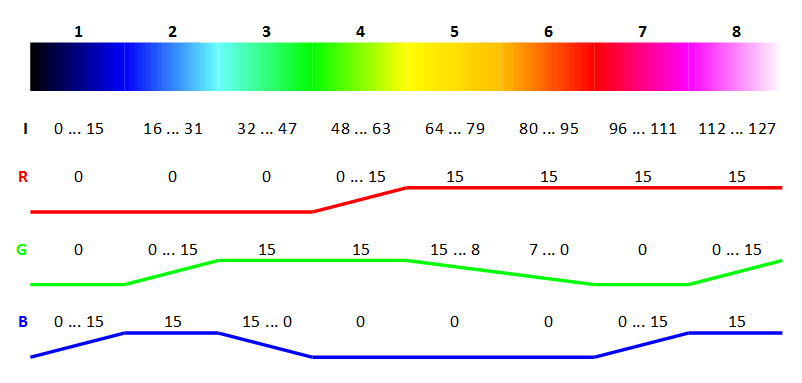
\includegraphics[width=\textwidth]{img/ColorScheme.png}
	\caption{Color distribution in $\qty{8}{\bit}$ according to the following scheme. The scheme is stretched from $\qty{7}{\bit}$ to $\qty{8}{\bit}$ to allow for finer color steps and to use 1 full byte.
	}
	\label{fig_color_scheme}
\end{figure}

\textbf{Brightness}

The brightness is sent as \qty{4}{\bit} value. The highest color component value is chosen and scaled with the brightness value to be relative to \qty{8}{\bit}. If two colors have the same highest brightness, the first is chosen.

For all other color components, their fragment of the brightest color is calculated and then scaled with the brightness value to be relative to \qty{8}{\bit}.
\FloatBarrier

\subsubsection{Config Frame}
There shall be one Frame, that can be used, to set various settings on the cone. This could be the ID or a command (eg. to turn the cone off). 
\begin{table}[h!]
	\centering
	\begin{zebratabular}{ccll}
		\rowcolor{gray}
		Byte & Size   		   & Name        	& Description\\
		0-15 & \qty{16}{\byte} & Header			& Header according to definition\\
		& & &\\	     
		16-17& \qty{2}{\byte}  & Parameter ID   & ID of parameter to be changed\\
		18-19& \qty{2}{\byte}  & Reserved		& Reserved to align data with 32 bit\\
		20-23& \qty{4}{\byte}  & Value  		& Value to be set\\	
	\end{zebratabular}
	\caption{Config Frame Definition}
	\label{tab_config_frame}
\end{table}
\FloatBarrier

\subsubsection{Settings/Status Request}
The Request Frame is used to request the Settings or status frame from a specific cone. When sent to the Broadcast address, all cones shall send a response. This frame does not contain any data. 
\begin{table}[h!]
\centering
\begin{zebratabular}{ccll}
	\rowcolor{gray}
	Byte & Size   		   & Name        	& Description\\
	0-15 & \qty{16}{\byte} & Header			& Header according to definition (Type 2 or 3)\\
\end{zebratabular}
\caption{Request Frame Definition}
\label{tab_request_frame}
\end{table}


\subsubsection{Settings Frame}
Due to low amount of configuration data of the cone, only all data can be requested. Each parameter uses \qty{8}{\byte}. 
\begin{table}[h!]
	\centering
	\begin{zebratabular}{ccll}
		\rowcolor{gray}
		Byte & Size   		   & Name        	& Description\\
		0-15 & \qty{16}{\byte} & Header			& Header according to definition\\
		& & &\\     
		16-17& \qty{2}{\byte}  & Parameter ID   & ID of parameter to be changed\\
		18-19& \qty{2}{\byte}  & Reserved		& Reserved to align data with 32 bit\\
		20-23& \qty{4}{\byte}  & Value  		& Value to be set\\	
		...&&&\\
	\end{zebratabular}
	\caption{Settings Frame Definition}
	\label{tab_settings_frame}
\end{table}

\subsubsection{Status Frame}
The status frame is periodically requested by the host and contains current status data as well as relevant Identification values. \todo{with presence of the Settings frame check if MAC Adress and revisions must be part of this frame}
\begin{table}[h!]
	\centering
	\begin{zebratabular}{ccll}
		\rowcolor{gray}
		Byte & Size   		   & Name        	& Description\\
		0-15 & \qty{16}{\byte} & Header			& Header according to definition\\
		& & &\\	     
		16-17& \qty{2}{\byte}  & ID  			& ID of the cone\\
		18   & \qty{1}{\byte}  & \ac{SoC}		& State of Charge scaled [\qtyrange[range-phrase=\textendash]{0}{100}{\percent}]\\
		19   & \qty{1}{\byte}  & \ac{RSSI} 		& \ac{RSSI} value scaled according to ESP\\	
		20-25& \qty{6}{\byte}  & \acs{MAC} Address& \ac{MAC} Address of the cone\\	
		26-27& \qty{2}{\byte}  & Software Rev	& Software Revision \qty{1}{\byte} for major, \qty{1}{\byte} for minor revision\\	
		28   & \qty{1}{\byte}  & Hardware Rev	& Hardware Revision \qty{4}{\bit} for major, \qty{4}{\bit} for minor revision\\	
		29   & \qty{1}{\byte}  & Hall Sensor	& Hall switch state [0/1]\\	
	\end{zebratabular}
	\caption{Status Frame Definition}
	\label{tab_settings_frame}
\end{table}



\FloatBarrier
\subsection{Logger}
The python module \texttt{Logging} is used for logging in the whole application. This makes it extremely simple to log any events. The logger is configured in the top module \texttt{LoggingManager}. The configuration itself is done using a \ac{JSON} formatted file. This file should be used by the user to tailor the logging behaviour if necessary. 
\subsubsection{HowTo Logging}
At least every large submodule as described above should have its own logger. If more loggers are needed, they can be created. Table  \ref{tab_logger} collects all loggers, that are created in the application. 
\begin{table}[h!]
	\centering
	\begin{zebratabular}{ll}
		\rowcolor{gray}
		Module &
		Logger Name \\
		Host-Network-Interface & NetworkInterface  \\
	\end{zebratabular}
	\caption{Logger Names}
	\label{tab_logger}
\end{table}

The logger can be created using \pythoninline{logger = logging.getLogger("your-best-logger-name")}. Creating messages is then pretty straight forward: 
\begin{python}
logger.debug("Debug message")
logger.info("Info message")
logger.warning("Warning message")
logger.error("Error message")
logger.critical("Critical message")
\end{python}

\subsubsection{LoggingManager}
The \texttt{LoggingManager} class together with the Handlers is used to filter and categorize the logger messages. 
\todo{Write Code and document it here}

\subsection{Host-Network-Interface}

This module is used to interface to any available network. It must be instantiated in the application. This allows to have multiple interfaces in parallel.

\subsubsection{Command line Interface}
The Module features a command line Interace, which can be used by running the python file \texttt{NetworkInterface.py}. The available options and corresponding functions can primarily be looked up using the \texttt{-h/--help} switch. Commands that need more explanation are explained hereinafter.  

\subsubsection{Defining the used network}
The module uses the \texttt{ifaddr} module for discovery of all available network interfaces. The returned list of type \texttt{ifaddr.Adapter} can be used to select the correct adapter. The adapter is selected by specifying the name and the used IP address. If the \ac{IP} address is not available, the first \ac{IP} address is used. 

\subsubsection{Network Operation}
The module has multiple threads, that can be launched to operate on the network interface. 

\textbf{Discovery Thread}\\
The discovery thread is used to collect data about all available cones. This includes only the periodic data (battery voltage, \ac{RSSI} etc). The data itself is buffered on the module, to allow access to it permanently. Each received message is pushed to the logger with level 

\textbf{Streaming Thread}\\
The streaming thread is used to send the current light state to all cones through a multicast message. This is done in the background. 
\todo{Define interface to get current light state from other application modules}

\subsubsection{\acs{UDP} Access}
One Thread is simply responsible to receive the packets.

\subsection{Network Manager}




\subsection{Scenario Designer}






\subsection{Simulator}



\subsection{Licensing}

As this software is intended to be made open source in near or far future, the license thematic is an important topic. Therefore all python dependencies are listed in the following table. 

\begin{table}[h!]
	\centering
	\begin{zebratabular}{llll}
		\rowcolor{gray}
		Module &
		pip install name & 
		License & url \\
		\texttt{ifaddr} & \texttt{ifaddr}  & MIT &  \url{https://github.com/pydron/ifaddr} \\
	\end{zebratabular}
	\caption{Python Dependencies} 	
	\label{tab_py_dependencies}
\end{table}


